
\newcommand{\commonfigurescomp}{Compression ratio and relative difference plots for $a_\maskalgo$ and $a_\NOmaskalgo$ for every\\coding algorithm $a \in A$, for the }

\begin{figure}
\hspace{-70pt}
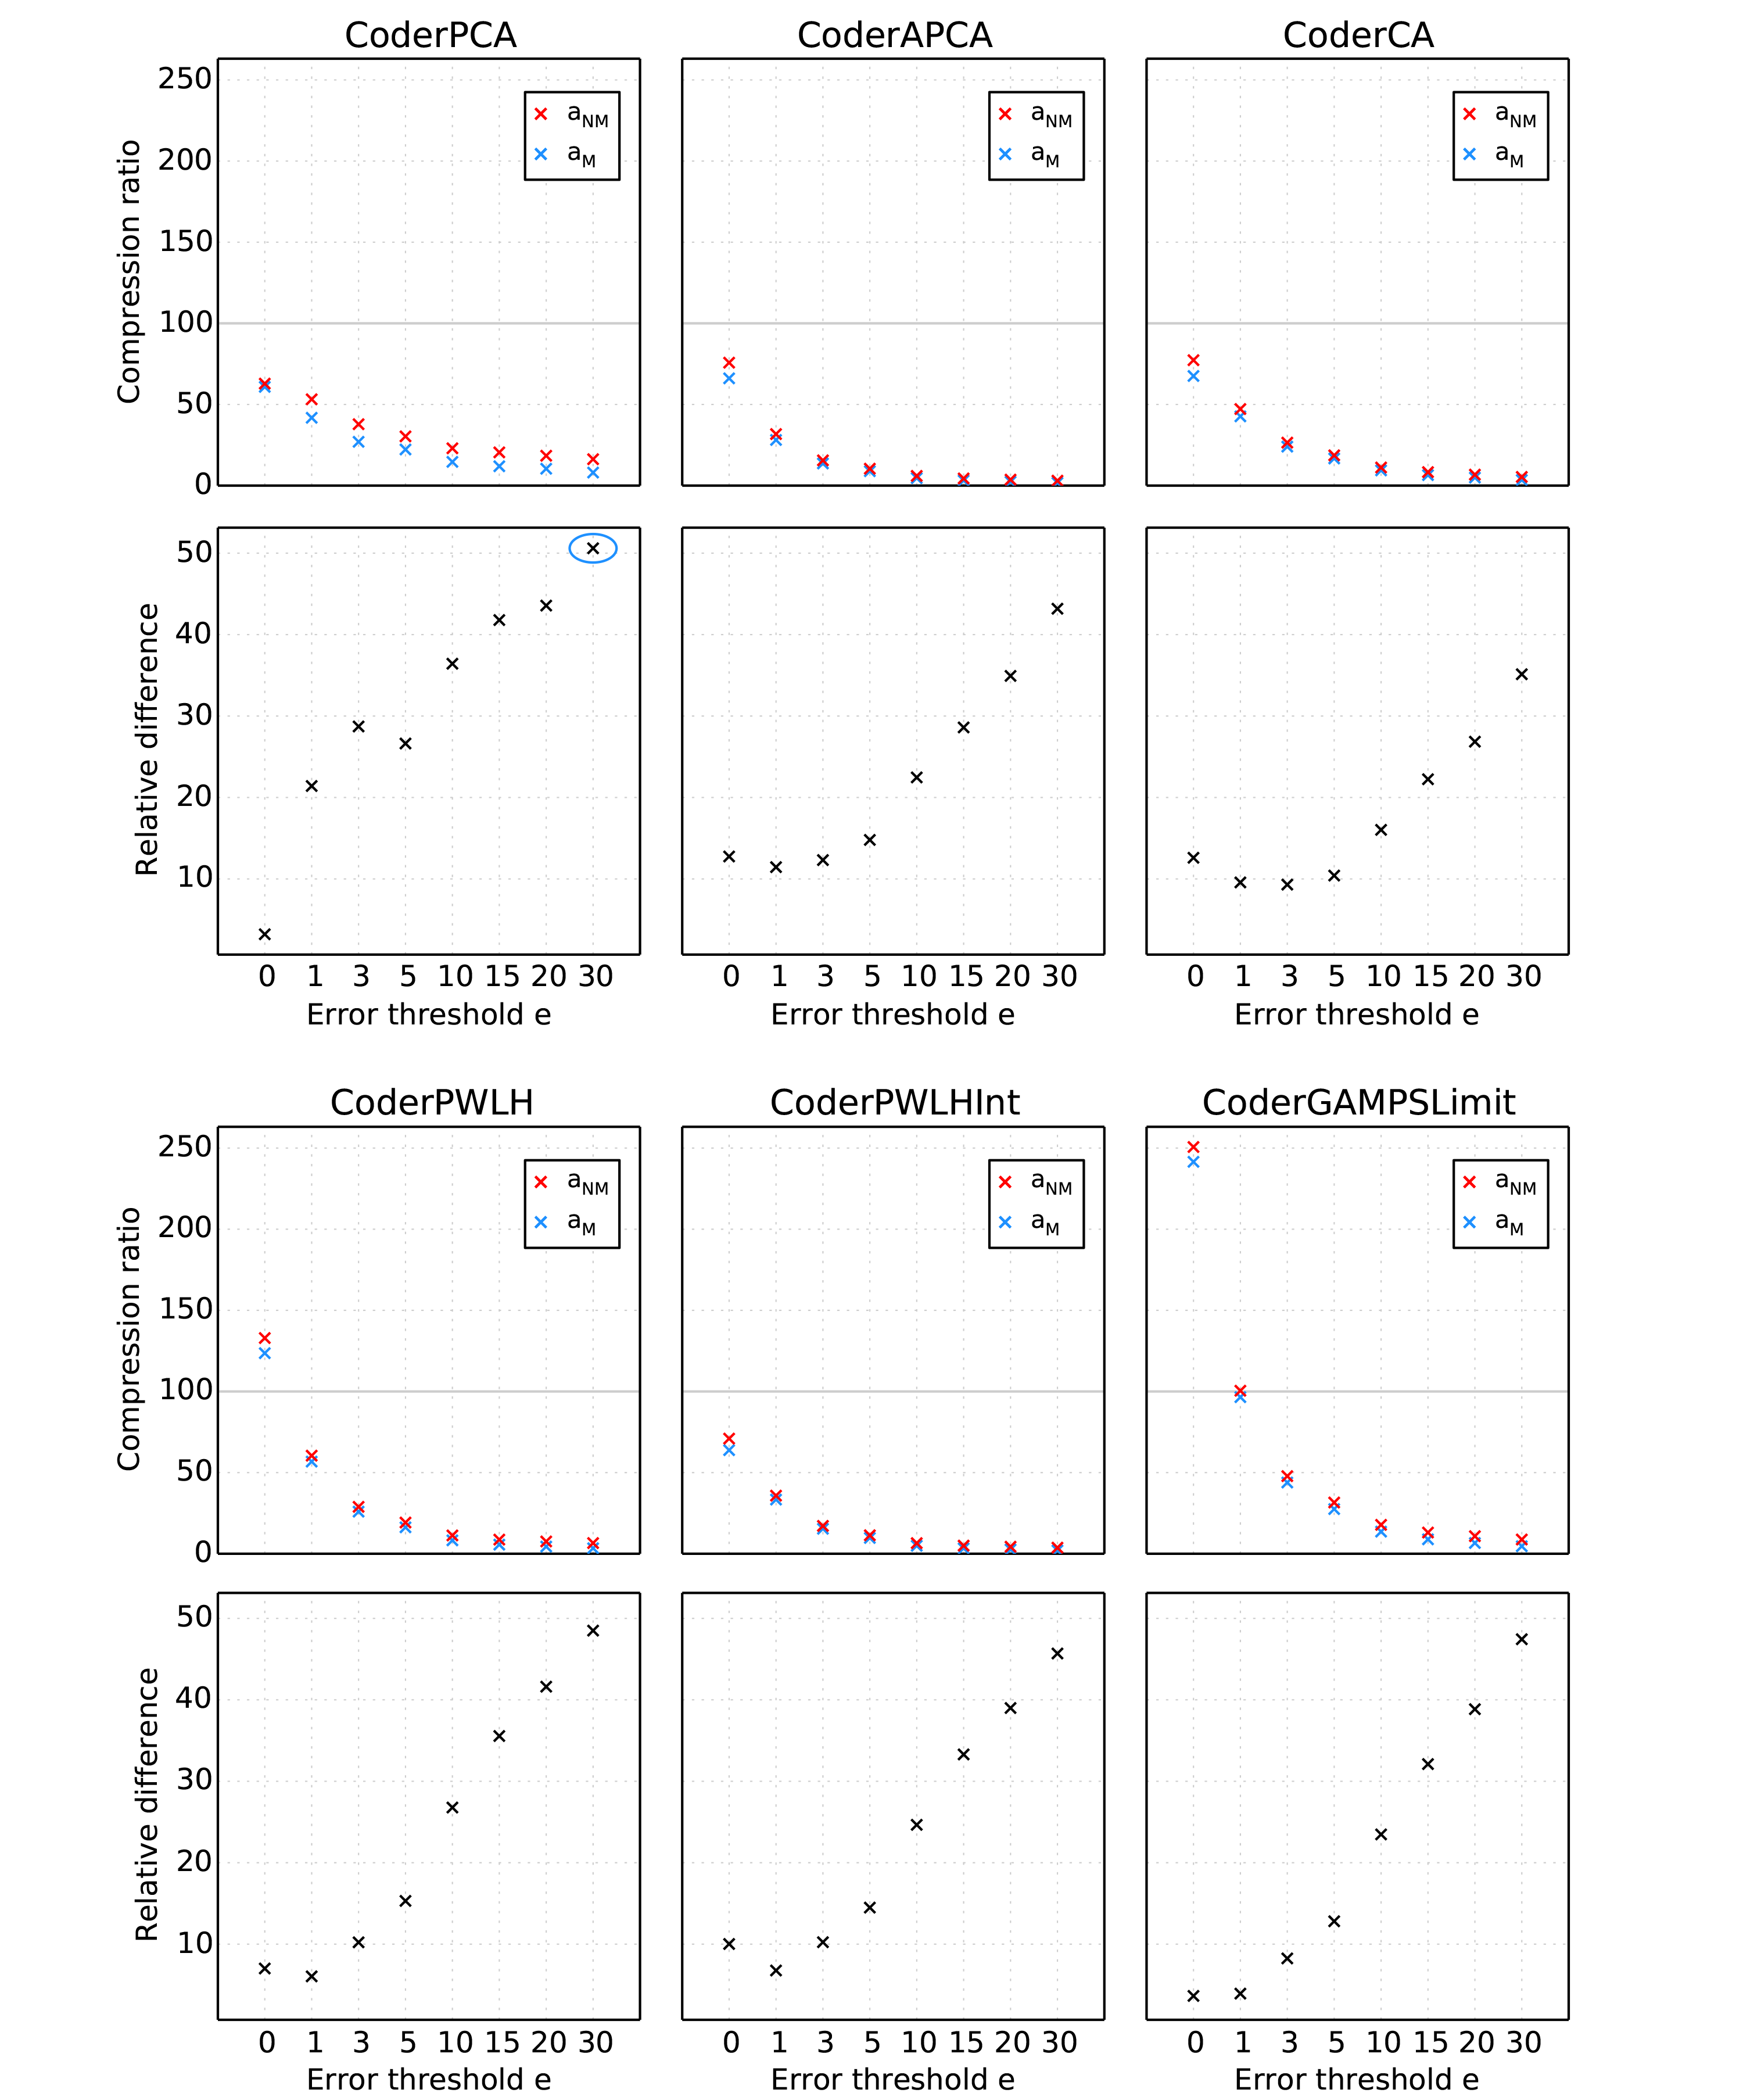
\includegraphics[scale=0.75]{chapters/Experiments/images/32-SST.png}
\hspace{+10pt}
\caption{\commonfigurescomp ``VWC" data type of the \datasetsst \ dataset.\\In the relative difference plot for CoderPCA we marked with a blue circle the case\\in which $a_\maskalgo$ obtains the most significant relative difference (50.60\%).}
\label{fig:diff-sst}
\end{figure}

\clearpage

\begin{figure}
\hspace{-70pt}
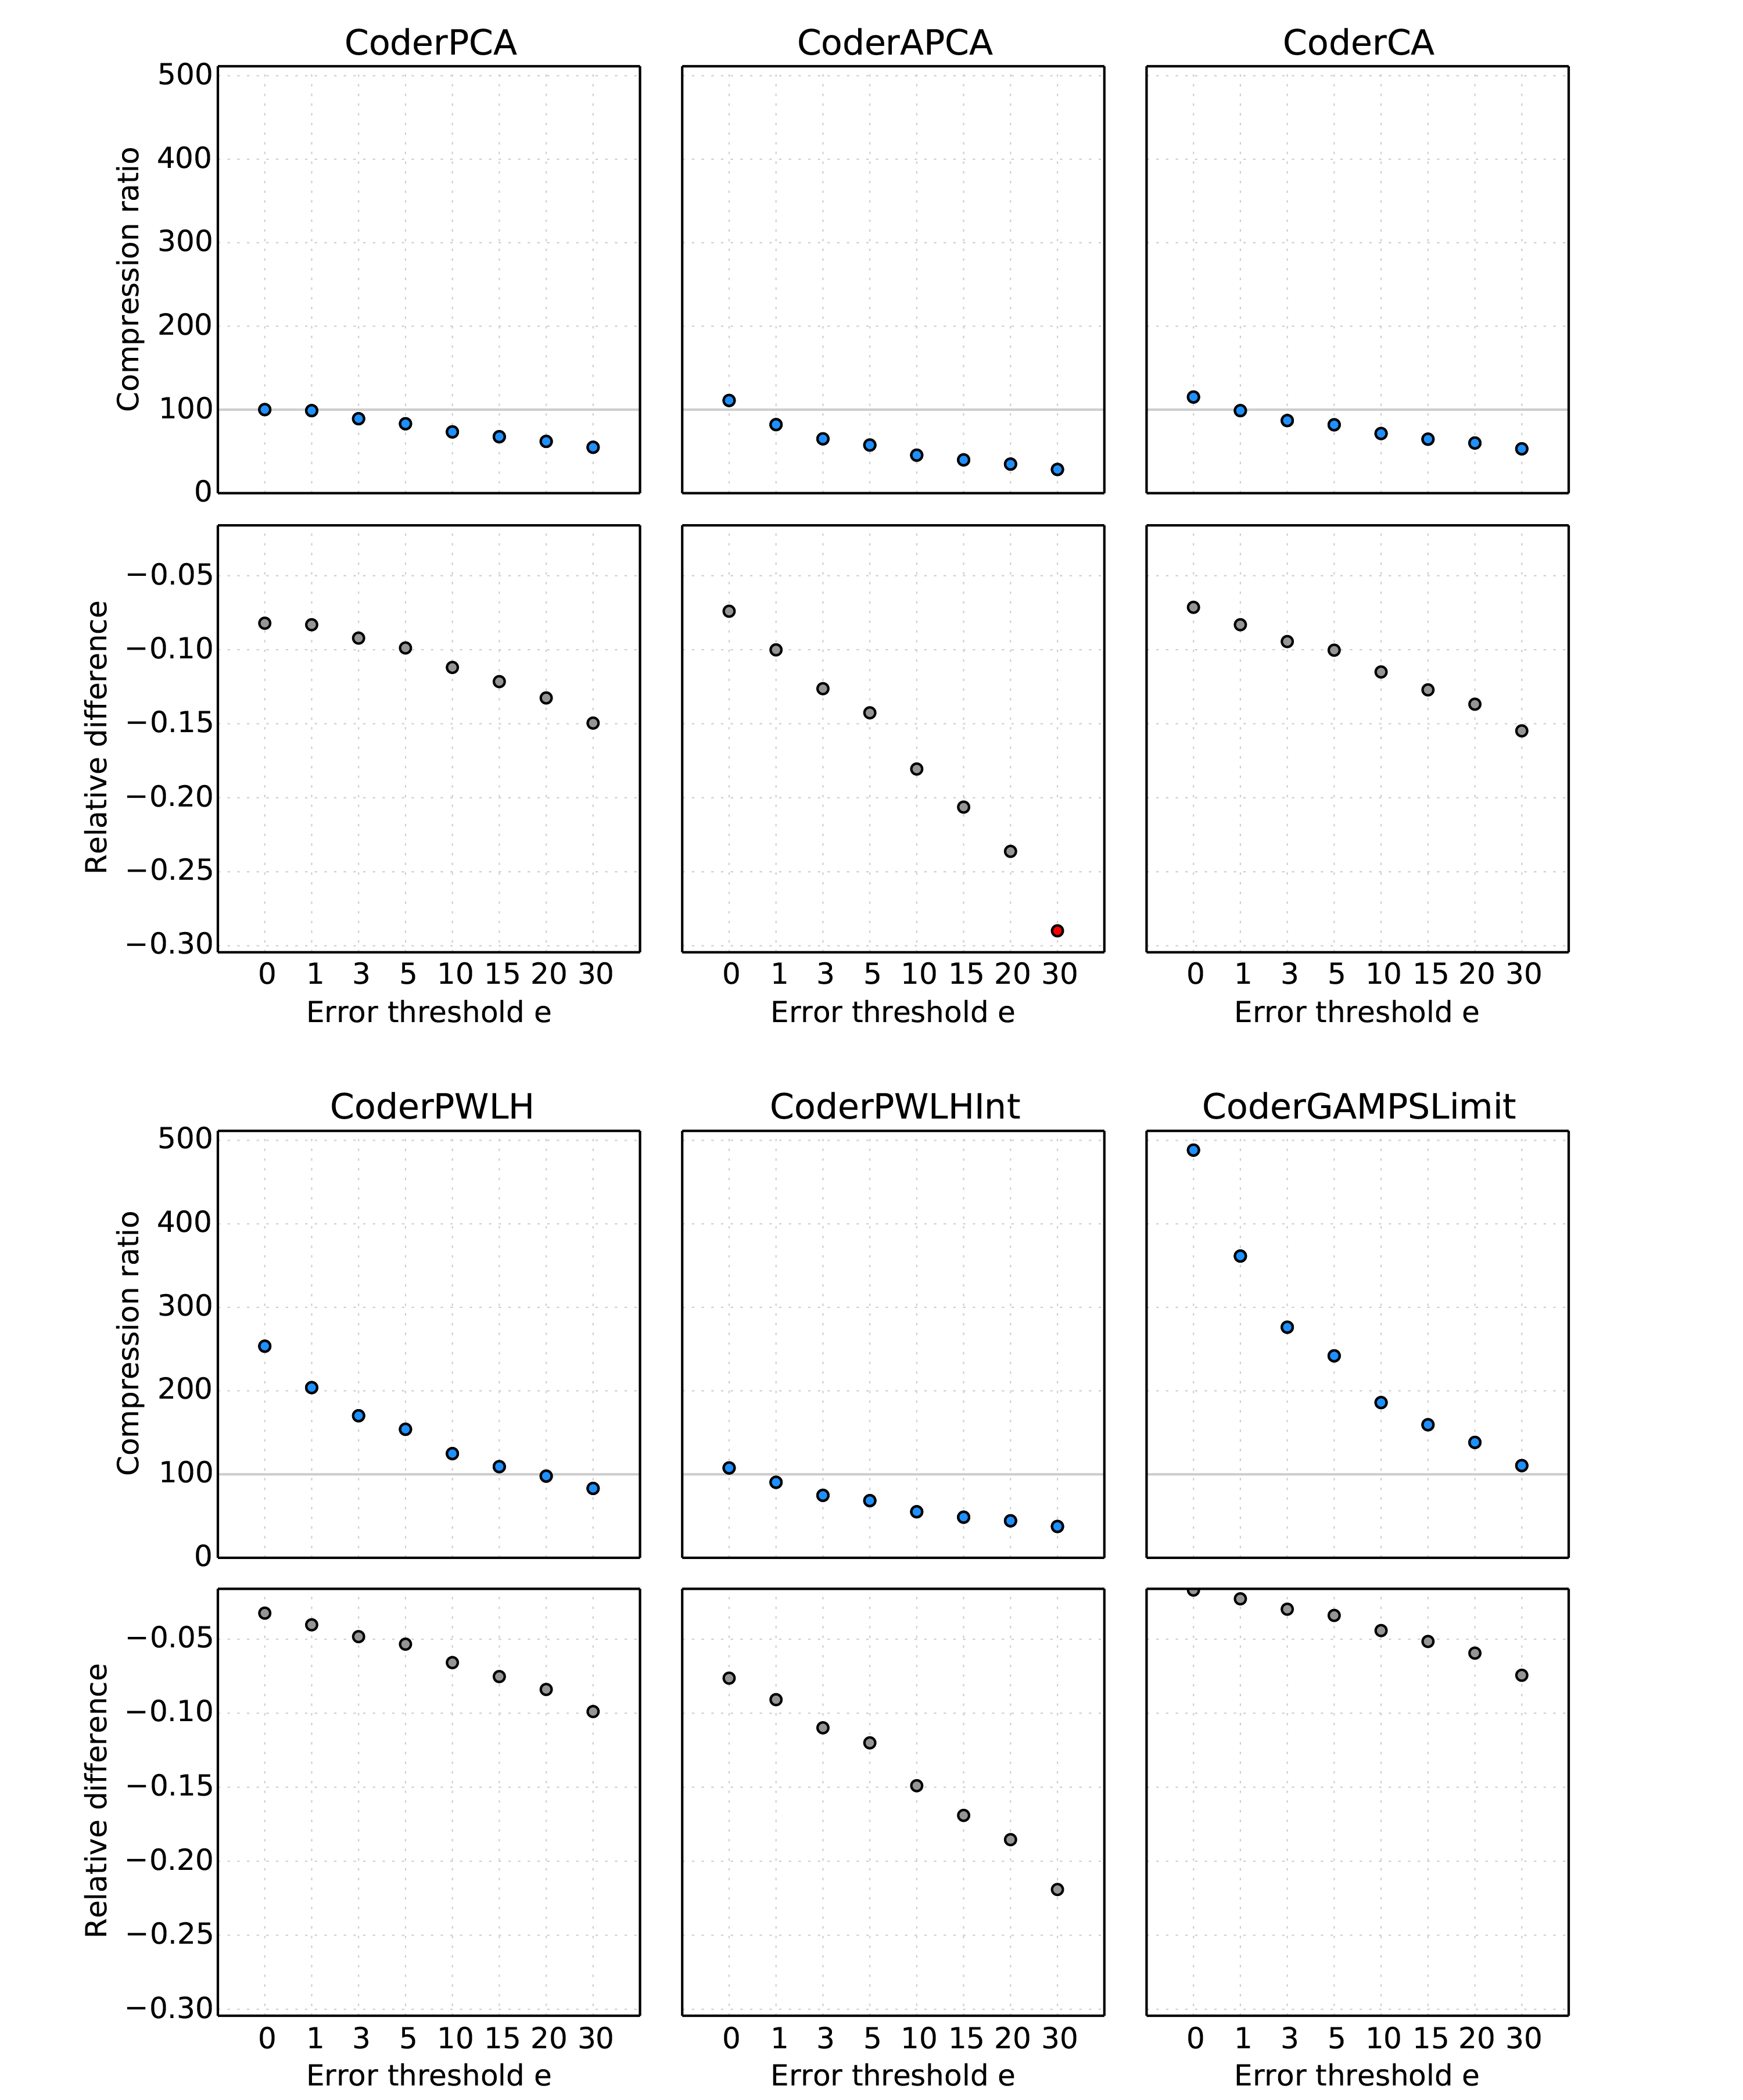
\includegraphics[scale=0.75]{chapters/Experiments/images/32-Tornado.png}
\hspace{+10pt}
\caption{\commonfigurescomp ``Longitude" data type of the \datasettornado \ dataset.\\In the compression ratio plot the red and blue markers are almost overlapping.\\In the relative difference plot for CoderAPCA we marked with a red circle the case\\in which $a_\NOmaskalgo$ obtains the most significant relative difference (-0.29\%).}
\label{fig:diff-tornado}
\end{figure}
